\chapter{Общая теория}
\section{Постановка задачи}
 

 Рассмотрим падение монохроматической плоской TM-волны на две полубесконечные металлические пластины (Рис.~\ref{fig:geom}). Мы рассматриваем однородную по оси  $y$ задачу, считая пластины бесконечными по этому направлению.
 Магнитное поле $H$ подчиняется однородному волновому уравнению 
 \begin{equation}
   \frac{\partial^2 H}{\partial x^2} +   \frac{\partial^2 H}{\partial z^2} = \frac{\epsilon}{c^2}\frac{\partial^2 H}{\partial t^2}.
 \end{equation}
 Здесь предполагается, что в инфракрасном диапазоне (длина волны $\lambda = 1,5$ мкм) золото немагнитное, то есть $\mu = 1$ и $B = H$. Область при $z<0$ 
 и между пластинами является вакуумом, и соответственно для него проницаемость $\eps_a = 1$, проницаемость металла является
 комплексной величиной $\eps = \eps' + i \eps''$, где вещественная часть $\eps'$ отрицательна и $\abs{\eps'} \gg 1$, мнимая же часть 
 отвечает за омические потери, следовательно положительна. 
\begin{figure}
\begin{center}
    
    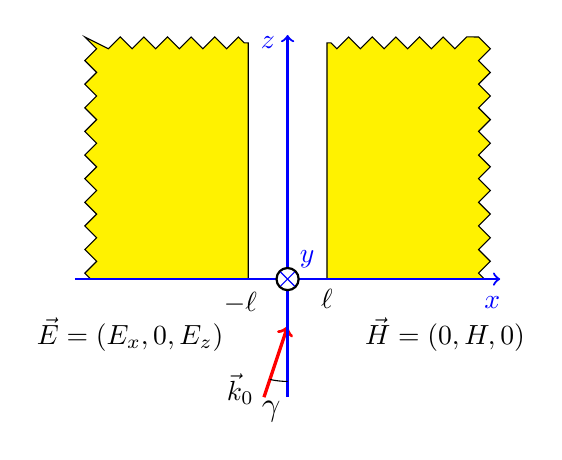
\begin{tikzpicture}[decoration={zigzag,segment length = 3mm, amplitude = 0.75mm}]
        \draw [very thick,red,->] (-0.3,-1.5)--(0,-0.6);
\draw [fill=yellow] (-2.5,0) decorate{--(-2.5,3) -- (-0.5,3)} -- (-0.5,0) -- cycle;
\draw [fill=yellow] (2.5,0) decorate{-- (2.5,3) -- (0.5,3)} -- (0.5,0) -- cycle;
        \draw [blue,thick,->] (-2.7,0)--(2.7,0);
        \draw [black] (0.5,-0.25) node {$\ell$};
        \draw [black] (-0.6,-0.3) node {$-\ell$};
        \draw [blue] (2.6,-0.3) node {$x$};
        \draw [blue,thick,->] (0,-1.5)--(0,3.1);
        \draw [blue] (-0.25,3) node {$z$};
        \draw [thick,fill=white] (0,0) circle (4pt);
        \draw [blue] (-0.09,-0.09)--(0.09,0.09);
        \draw [blue] (0.09,-0.09)--(-0.09,0.09);
        \draw [blue] (0.25,0.25) node {$y$};
        \draw (-0.6,-1.4) node {$\vec{k}_0$};
        \draw (2.0,-0.7) node {$\vec{H} = (0,H,0)$};
        \draw (-2.0,-0.7) node {$\vec{E} = (E_x,0,E_z)$};
        \draw (0,-1.3) arc (-90:-103:1);
        \node[] at (263:1.7)  {\large$\gamma$};
        \end{tikzpicture}
\end{center}
\caption{Геометрия задачи.}
\label{fig:geom}
\end{figure}

Так как падающее излучение монохроматично, мы будем искать прошедшую в щель и рассеянную на ней волны в том же виде 
$f(t) \sim e^{-i \omega t}$, таким образом, задача сводится к решению однородного уравнения Гельмгольца
 \begin{equation}
   \label{eq:Helmholtz}
   \frac{\partial^2 H}{\partial x^2} +   \frac{\partial^2 H}{\partial z^2} + \eps k_0^2 H = 0,
 \end{equation}
где $k_0 = \omega/c$ --- волновое число падающей волны. 

Мы будем искать решение в комплексной форме $h(x,z,t) = H(x,z)e^{-i \omega t}$, а настоящее поле является суммой решения и его комплексного сопряжения $H(x,z)e^{-i \omega t} + \text{к. с.}$

\section{Решение в полупространствах}
Выберем систему координат как показано на Рис.~\ref{fig:geom}. Область $z > 0$ состоит из двух бесконечных в направлении $y$ и полубесконечных в направлении $x$ подобластей из золота и щели между ними. Пусть центр щели будет расположен при $x = 0$, а ширина равна $2\ell$. Плоская монохроматическая волна TM поляризации падает из нижнего полупространства $z<0$ с волновым вектором, ориентированным под углом $\gamma$ к базисному вектору $\mathbf{e}_z$. Будем говорить, что рассматривается нормальное падение на щель, когда угол $\gamma = 0$.

 Для нахождения распределения магнитного поля достаточно найти общие решения волнового уравнения в обоих полупространствах $z>0$ и $z<0$, а затем их сшить при $z = 0$, используя непрерывность полей $\mathbf{E}$ и $\mathbf{H}$. Так как граница $z=0$ неоднородна из-за наличия щели в области
 $\abs{x} < l$, искать решение удобнее всего, разделяя переменные, как в работах \cite{sturman2010transmission,gorkunov2011transmission}, 
 явным образом выделяя часть, 
 зависящую от $x$. Рассмотрим поля в каждом из подпространств по отдельности.

 \subsubsection{Поле в области $z < 0$}
 
В силу линейности уравнения~(\ref{eq:Helmholtz}), решение удобно искать в виде интеграла Фурье

\begin{equation}
  H^<(x,z) = (e^{i k_{0z} z} + R e^{-i k_{0z} z}) e^{i k_{0x} x} + \int a_k e^{i (k x - \varkappa z)} dk, 
\end{equation}
где первый член отвечает обычному отражению плоской TM волны от плоской границы с коэффициентом Френеля 
\[
 R = \frac{\eps \cos{\gamma} - \sqrt{\eps - \sin^2{\gamma}}}{\eps \cos{\gamma} + \sqrt{\eps - \sin^2{\gamma}}}
\]
для данного угла падения $\gamma$.  
Второй член отвечает волне, рассеянной на щели, и представляет собой интеграл по всем плоским волнам. Величина $\varkappa = \sqrt{k_0^2-k^2}$ является
$z$ компонентой волнового вектора рассеянной волны, которой соответствует амплитуда $a_k$. Волны с $\abs{k} < k_0$ являются распространяющимися,
а волны с большим по модулю $k$ затухают экспоненциально при удалении от щели (такие волны также называют эванесцентными). Подобный выбор формы решения удобен в процессе сшивки при $z = 0$, так как в коэффициенте отражения $R$ уже учтены граничные условия для падающей и отраженной волны, что позволяет напрямую связать амплитуды рассеянных гармоник $a_k$ с возбуждаемыми модами в щели. 

\subsubsection{Поле в области $z>0$}
Рассмотрим в первую очередь область внутри щели $\abs{x}<\ell$. Разделяя переменные, локализованное внутри щели решение 
находим в виде ряда Фурье 
\begin{equation}
H^>(x,z) = \sum_{\nu = -\infty}^{\infty} h_\nu m_\nu(x) e^{i \beta_{\nu} z},
  \label{eq:Fourier_series}
\end{equation}
где константа распространения $\beta_\nu^2 =  k_0^2-q_\nu^2 $ определяет, какие моды являются распространяющимися в щели, а какие эванесцентными. Величина $q_\nu$ называется собственным значением моды $\nu$. 
По сути, как это будет видно впоследствии, мнимая и вещественная части $\beta_\nu$ определяют, какие гармоники дают вклад в плазмонную силу. 

Функции $m_\nu(x)$ являются 
решением уравнения 
\begin{align}
  m''_\nu(x) + q_{\nu}^{2}m_\nu(x) = 0, & \ \abs{x}<\ell, \\
  q_\nu^2 = k_{0}^{2}-\beta_\nu^{2}.& \nonumber
\end{align}
Решением данного уравнения являются тригонометрические функции $m_\nu(x) = \cos(q_\nu x) \ (\sin(q_\nu x))$ для чётных (нечётных) $\nu$. Значение $q_\nu$ для каждой моды получается из сшивки
магнитного и электрического полей на границе щели.
Аналогично поиску локализованных мод в работе~\cite{sturman2007eigenmodes}, для магнитного поля в металле мы ищем затухающее на бесконечности решение $m_\nu^M(x)$, которое подчиняется уравнению
\begin{align}
  (m^M_\nu(x))'' - q_{M_\nu}^{2}m^M_\nu(x) = 0, & \ \abs{x}>\ell, \\
  q_{M_\nu}^{2} = \beta_\nu^{2}-\eps k_{0}^{2}. &\nonumber
\end{align}
Решением этого уравнения является затухающая экспонента $T e^{-(x-\ell)q_{M_\nu} }$ (для $x>0$). 
Из уравнений Максвелла мы знаем, что $E_z \sim (1/\eps) \partial_x H$, таким образом граничные условия непрерывности полей дают следующую систему уравнений для чётных мод 
\begin{equation}
    \begin{cases}
        \cos(q_\nu \ell) = T, \\
        q_\nu \sin (q_\nu \ell)  = \frac{T}{\eps} q_{M_\nu},
    \end{cases}
\end{equation}
и для нечётных
\begin{equation}
    \begin{cases}
        \sin(q_\nu \ell) = T, \\
        -q_\nu \cos (q_\nu \ell)  = \frac{T}{\eps} q_{M_\nu}. 
    \end{cases}
\end{equation}
Исключая $T$ из уравнений (см. Приложение А), мы получаем дисперсионное уравнение на $q_\nu$, которое можно переписать в экспоненциальной форме
\begin{align}
e^{2i q_\nu \ell} &= \pm \frac{i-g(q_\nu,\varepsilon)}{i+g(q_\nu,\varepsilon)},\label{eq:BoundCond} \\
g(q_\nu,\varepsilon) & = \frac{\sqrt{(1-\varepsilon)(k_0 \ell)^2 - (q_\nu \ell)^2}}{\varepsilon q_\nu \ell}.  \nonumber
\end{align}
Здесь знак <<$+$>> соответствует чётным модам, а <<$-$>> нечётным. Это уравнение трансцендентное, следовательно найти точное аналитическое решение
для всех мод невозможно. Однако есть возможность найти приближённое решение при  $\abs{\varepsilon} \gg 1$ и проанализировать поведение корней в предельном случае $\eps \to -\infty$, что соответствует идеальному проводнику.

Для простоты пренебрежём омическими потерями ($\eps'' = 0$). Раскладывая функцию $g(q_\nu,\varepsilon)$ в ряд Тейлора по $1/\varepsilon$ до первого члена мы получаем
\begin{equation*}
g(q_\nu,\varepsilon) = -\frac{k_0 \ell}{\sqrt{\abs{\varepsilon}}q_\nu \ell} + O\Big(\frac{1}{\abs{\varepsilon}^{3/2}}\Big),
\end{equation*}
откуда уравнение~(\ref{eq:BoundCond}) преобразуется в форму
\begin{equation}
e^{2i q_\nu \ell} \approx \pm\left(1 - 2i\frac{k_0 \ell}{\sqrt{\abs{\varepsilon}} q_\nu \ell}\right).
\label{eq:BoundCond_simple}
\end{equation}
Приближённое решение этого уравнения можно уже найти итеративно, если учесть что при $\varepsilon \to -\infty$ собственные значения
$q_\nu$ стремятся к $\frac{\pi \nu}{2 \ell}$.
\begin{align}
q_\nu^2  = -\frac{k_0}{ \sqrt{\abs{\varepsilon}} \ell}, &\ \nu = 0; \nonumber \\
q_\nu \ell = \frac{\pi \nu}{2} - \frac{2k_0\ell}{\pi \nu \sqrt{\abs{\varepsilon}}}, &\ \nu = \pm 1,\pm 2,\pm 3...\label{eq:Eigenvalues_approx}
\end{align}
\begin{figure}
    \begin{center}
    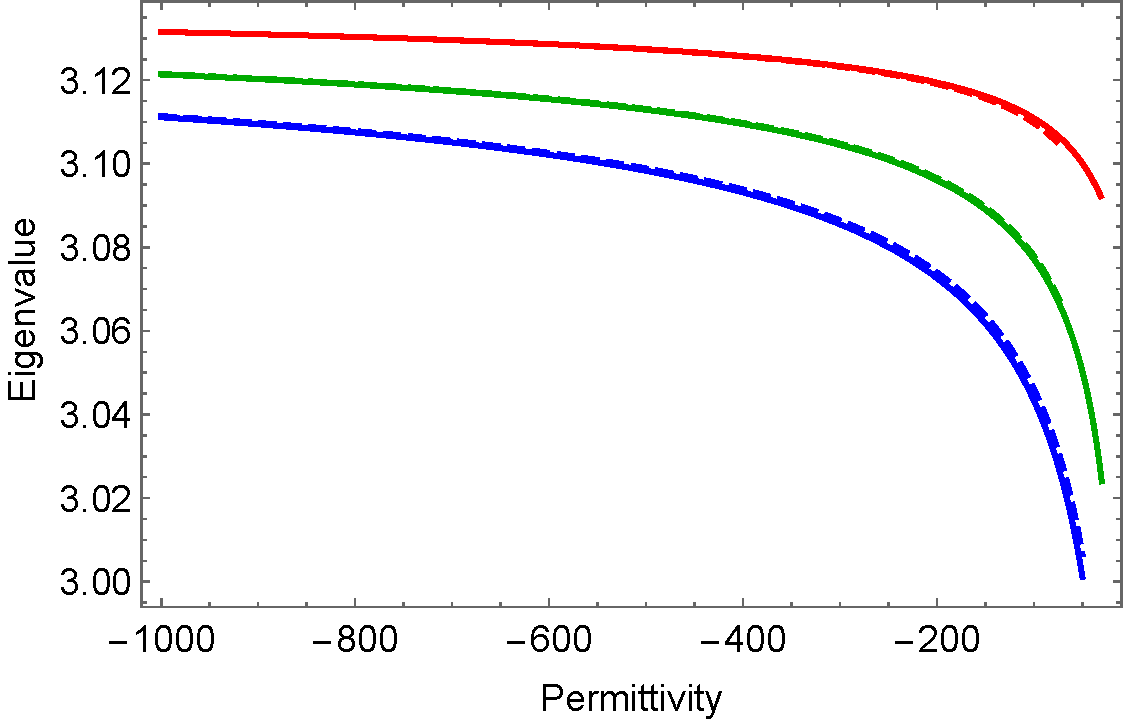
\includegraphics[width=1.0\columnwidth]{2nd_eps.pdf}
      \caption{Зависимость собственного значения $q_2\ell$ от диэлектрической проницаемости $\eps$ при $k_0 \ell = 1,2,3$ (сверху вниз):
      численный счёт (сплошная линия), асимптотическая формула (пунктирная линия).}
      \label{fig:2nd_mode}
    \end{center}
\end{figure}
\begin{figure}
    \centering
    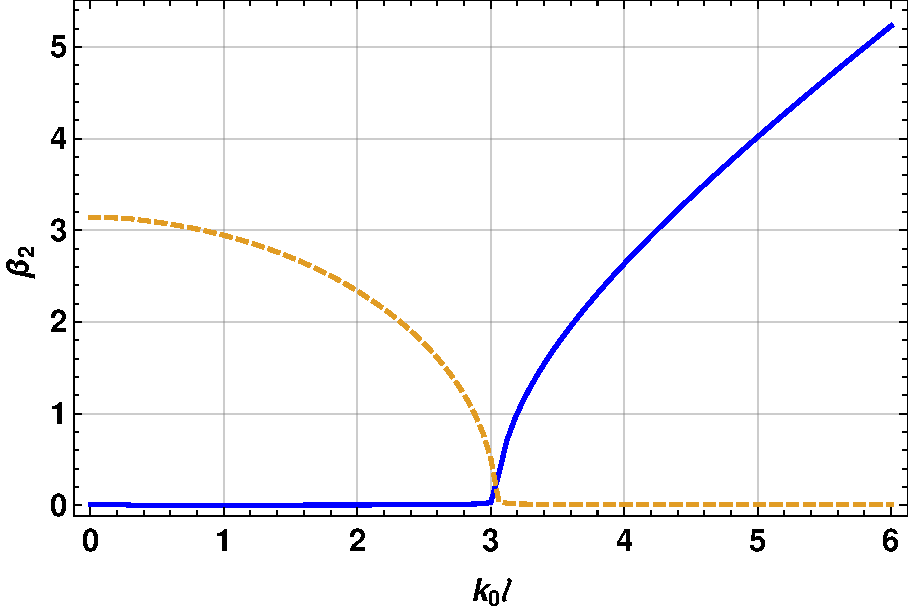
\includegraphics[width=1.0\columnwidth]{figures/betta2_real.pdf}
    \caption{Зависимость константы распространения 
      $\beta_2$ при $\eps = -100+10i$ в зависимости от безразмерной ширины щели $k_0\ell$: вещественная часть (сплошная кривая), мнимая часть (штрихпунктир).}
    \label{fig:betta2}
\end{figure}
Здесь чётные и нечётные $\nu$ соответствуют чётным и нечётным модам. Как и должно быть, главный член по $\eps$ отвечает решению для идеального
проводника, в то время когда поправка имеет порядок $O(\abs{\varepsilon}^{-1/2})$ для всех мод кроме фундаментальной $\nu = 0$, для 
неё $q_0 \sim \abs{\varepsilon}^{-1/4}$. Рассмотрим частный случай сравнения расчёта одного собственного значения
полученного численным образом и приближённой формулой. На Рис.~\ref{fig:2nd_mode} представлена зависимость собственного значения $q_2\ell$ от 
диэлектрической проницаемости  $\eps$ для различных значений параметра $k_0 \ell = 1,2,3$, которая найдена численно и с использованием
приближённого выражения~(\ref{eq:Eigenvalues_approx}). Можно заметить, что разница между точным значением и приближённым возрастает с ростом  $k_0 \ell$, а при увеличении $\abs{\varepsilon}$ значения сходятся к $\pi$, чего и следовало ожидать. 

 При $\varepsilon'' \neq 0$, значение $q_\nu$ становится комплексной величиной, а соответствующая константа 
 распространения $\beta_\nu$ приобретает положительную мнимую часть и для распространяющихся мод в щели (см. Рис.\ref{fig:betta2}). Мнимая часть $\beta_\nu''$ определяет
 глубину проникновения моды $\nu$ в щель, так как $\abs{h_\nu(z)}\sim e^{-\beta_\nu'' z}$. Как только длина пластин $L_z$ вдоль оси $z$ становится много больше, чем характерная длина проникновения, то 
 есть $L_z \gg 1/\beta_\nu''$, мы можем пренебречь френелевским отражением от границы $z = L_z$ и рассматривать только моду, распространяющуюся внутрь щели.  Как только $1/\min \limits_{\nu}(\beta_\nu'') \ll L_z$,
 то длиной щели можно пренебречь. 

\section{Тензор Максвелла}

Давление электромагнитного поля можно описать с помощью тензора натяжений Максвелла~\cite{landau}.  \begin{equation*}
  \sigma_{\alpha \beta}(t) = \frac{1}{4 \pi}\Big( E_\alpha(t) E_\beta(t) + H_\alpha(t) H_\beta(t) - \frac{1}{2}\delta_{\alpha \beta}(E^2(t) + H^2(t)) \Big).
\end{equation*} Нас интересует давление электромагнитного поля по оси $x$ в точках $x = \pm \ell$
\begin{equation*}
    \sigma_{xx}(t) = \frac{1}{8 \pi}\Big( E_x^2(t) - E_z^2(t) - H_y^2(t)\Big).
\end{equation*}
Используя, что $E_{i}(t) = E_i e^{-i \omega t} + \text{к. с.}$, усреднением тензора Максвелла по периоду получаем следующий результат
\begin{equation}
    \sigma_{xx} = \frac{1}{4 \pi} (\abs{E_x}^2 -\abs{E_z}^2 - \abs{H_y}^2).
\end{equation}

Рассмотрим ситуацию, когда в щели возбуждена лишь одна мода с индексом $\nu$, тогда поля
\begin{align*}
    H_y &= h_\nu m_\nu(\ell) e^{i \beta_\nu z},  \\
    E_z &= \frac{i}{k_0} q_\nu h_\nu m_\nu'(\ell) e^{i \beta_\nu z},  \\
    E_x &= \frac{1}{k_0} \beta_\nu h_\nu m_\nu(\ell) e^{i \beta_\nu z},
\end{align*}
где $m_\nu'(\ell)$ означает производную функции $\cos(\mathrm{x}) \ (\sin(\mathrm{x}))$ в точке $\mathrm{x}= q_\nu \ell$. 
Предполагая, что $\abs{\eps'} \gg 1$, мы можем пренебречь $E_z$ (так как $q_\nu \ell \to \pi \nu/2$, $m_\nu(\ell) \to 1 $ и $m_\nu'(\ell) \to 0$ при $\eps \to -\infty$), тогда давление будет иметь вид
\begin{equation}
   \sigma_{xx} \approx \frac{\abs{h_\nu}^2}{4 \pi k_0^2}(\abs{\beta_\nu}^2 - k_0^2 )e^{-2\beta_\nu'' z}.
   \label{eq:F_fund_mode_SGS}
\end{equation}
Интегрируя данное выражение по всей поверхности щели, мы получаем вклад одной гармоники в плазмонную силу на единицу длины вдоль оси $y$
\begin{equation}
  F \approx \frac{\abs{h_\nu}^2}{8 \pi \beta_\nu'' k_0^2} (\abs{\beta_\nu}^2 - k_0^2),
  \label{eq:F_fund_mode_SI}
\end{equation}
Отсюда видно, что притяжение обусловливает лишь фундаментальная мода $\nu = 0$, ведь только для неё $\abs{\beta_0} > k_0$, для других мод это неравенство имеет обратный знак. 
Более того, мнимая часть константы распространения $\beta_\nu''$ прямым образом определяет величину силы, так как она характеризует глубину проникновения моды в щель; кроме того, определяющий вклад в силу будут давать распространяющиеся моды, а вклад эванесцентных будет подавлен.

Если предположить, что в щели возбуждается лишь фундаментальная мода, что соответствует субволновой ширине щели $k_0 \ell \ll 1$, то можно найти приближённое выражение для $\beta_0$. Это было проделано в работе~\cite{Frumin11} в пределе $\eps'' \ll \abs{\eps'}$. Авторы получили 
выражение
\begin{align}
    \beta_0' &= k_0 + \frac{k_0}{2 \sqrt{\abs{\varepsilon'}}k_0 \ell},  \\
    \beta_0'' &= \frac{1}{4}\frac{\varepsilon''}{\abs{\varepsilon'}^{3/2}\ell}.
\end{align}
Тогда выражение для силы на единицу длины приобретает следующий вид
\begin{equation}
    F \approx \frac{1}{4\pi}\frac{\abs{h_0}^2 \lambda}{\pi}\frac{\abs{\eps'}}{\eps''},
\end{equation}
или в системе СИ
\begin{equation}
    F \approx \mu_0\frac{\abs{h_0}^2 \lambda}{\pi}\frac{\abs{\eps'}}{\eps''}.
\end{equation}

Из-за неровностей пластин в эксперименте достичь расстояния меньше, чем длина волны не удаётся. Таким образом, в щели может возбуждаться произвольное количество мод, и значит поле представляет собой сумму по всем модам 
\begin{equation*}
H_y = \sum_{\nu} h_\nu m_\nu(\ell) e^{i \beta_\nu z},
\end{equation*}
\begin{equation*}
E_x = \frac{-i}{k_0}\frac{\partial H_y}{\partial z} = \frac{1}{k_0}\sum_{\nu}\beta_\nu h_\nu m_\nu(\ell) e^{i \beta_\nu z},
\end{equation*}
\begin{equation*}
E_z = \frac{i}{k_0}\frac{\partial H_y}{\partial x} = \frac{i}{k_0}\sum_{\nu} q_\nu h_\nu  m'_\nu(\ell) e^{i \beta_\nu z},
\end{equation*}
и тогда вклад в силу будут давать не только каждая из гармоник по отдельности, но и интерференционные члены между ними. Однако можно заранее сказать, что вклад от затухающих мод будет пренебрежим, по сравнению с распространяющимися. 

\section{Сшивка полей для плоской волны}

 Граничные условия при $z = 0$ для тангенциальной составляющей полей $E_x^<(x,0) = E_x^>(x,0) $ и $H_y^<(x,0) = H_y^>(x,0)$ 
 позволяют найти неизвестные $a_k$ и $h_\nu$.  Из этих условий следуют уравнения 
\begin{align}
\sum_{\nu = -\infty}^{+\infty} h_\nu m_\nu (x) = (1+R)e^{ik_{0x}x} 
+ \int a_{k'} e^{ik'x} dk', & \ \abs{x}<\ell, \label{eq:H} \\
\sum_{\nu = -\infty}^{+\infty} \beta_\nu h_\nu m_\nu(x) = (1-R)k_{0z}e^{ik_{0x}x}
- \int \varkappa a_{k'} e^{ik'x} dk', &\ \abs{x}<\ell,  \label{eq:Ex_in} \\
  \sum_{\nu = -\infty}^{+\infty} c_\nu(x)\beta_\nu h_\nu m_\nu(\ell) e^{-q_{M\nu}\abs{x-\text{sign}(x)\ell}} = 
 -\eps \int \varkappa a_{k'} e^{ik'x} dk', &\ \abs{x}>\ell. \label{eq:Ex_out}
\end{align}
Где коэффициент $c_\nu(x)$ равен единице для чётных мод и $\text{sign}(x)$ для нечётных, $q_{M\nu}^2 = \beta_\nu^2 - \eps k_0^2$
соответствует собственному значению моды $\nu$ в металле, и по сути является просто обратной длиной проникновения в стенки, так как 
является показателем в затухающей экспоненте. Уравнение~(\ref{eq:H}) обеспечивает непрерывность поля $H$ на входе в щель, 
уравнения~(\ref{eq:Ex_in}) и~(\ref{eq:Ex_out}) обеспечивают непрерывность тангенциальной компоненты $E_x \sim \partial_{z} H_y$ при $z = 0$. Следует отметить, что в уравнении~(\ref{eq:Ex_out}) в обеих частях отсутствует член, связанный с падающей волной. Связано это с тем, что выбранное нам решение для падающей волны автоматически удовлетворяет граничным условиям непрерывности на границе с металлом благодаря френелевским коэффициентам отражения и прохождения.  

Умножая уравнения~(\ref{eq:Ex_in}) и~(\ref{eq:Ex_out}) на $e^{-ikx}$и интегрируя от $x = -\infty$ до $x = +\infty$  
мы выражаем $a_k$ через $h_\nu$:
\begin{align}
a_k = \frac{k_{0z}\ell }{\pi \varkappa} (1-R)\sinc((k_{0x}-k)\ell) 
        - \frac{\ell}{2 \pi \varkappa}\sum_{\nu = -\infty}^{+\infty} \beta_\nu h_\nu\left[f_{q_\nu,k}
+ \frac{m_\nu(\ell)}{\eps}G(q_\nu,k)\right],
\end{align}
где $f_{q_\nu,k}$ и $G(q_\nu,k)$ определены следующим образом:  для чётных мод
\begin{align*}
&f_{q_\nu,k} =
\sinc(q_\nu-k)\ell + \sinc(q_\nu+k)\ell,\\
&G(q,k) = 2\frac{q\cos{k\ell}+k\sin{k\ell}}{q^2 + k^2}\\
\end{align*}
и для нечётных
\begin{align}
&f_{q_\nu,k} = i\ \sinc(q_\nu-k)\ell - i\ \sinc(q_\nu+k)\ell,\nonumber\\
& G(q,k) = -2\frac{q\sin{k\ell}+k\cos{k\ell}}{q^2 + k^2}.
\end{align}
Здесь использовано обозначение  $\sinc(x) = {\sin{x}}/{x}$.

Теперь мы подставляем $a_k$ в уравнение~(\ref{eq:H}), чтобы найти $h_\nu$. Умножая полученное уравнение на  $\cos{q_\mu x}$ ($\sin{q_\mu x}$) 
и интегрируя по $x$ от $-\ell$ до $\ell$, мы получаем систему линейных уравнений на $h_\nu$. Благодаря разным чётностям функций $\sin$ и $\cos$  полная система
разбивается на две независимые для чётных и нечётных по отдельности. Система уравнений на коэффициенты при чётных модах 
\begin{align}
	\sum_{\nu=-\infty}^{+\infty} F_{\mu \nu} h_\nu = (1+R)f_{q_\mu,-k_{0x}} + \frac{(1-R)k_{0z} \ell}{\pi}\int f_{q_\mu,-k}\sinc((k_{0x}-k)\ell) \frac{dk}{\varkappa}; \label{eq:General_System}
\end{align}
где 
\begin{align}
F_{\mu \nu} &= f_{q_\mu,q_\nu} + \frac{\beta_\nu}{2\pi}\int
\Bigl(f_{q_\nu,k}f_{q_\mu,-k}  + \frac{m_\nu(\ell)}{\eps} G(q_{M\nu},k)f_{q_\mu,-k} \Bigr)\frac{dk}{\varkappa}.
\label{eq:F_mn}
\end{align}
Для нечётных мод нужно лишь умножить первый член $f_{q_\mu,q_\nu}$ в уравнении~(\ref{eq:F_mn}) на $-i$ и взять соответствующие нечётные функции. Эта система уже позволяет анализировать по отдельности эффекты непараллельного падения излучения на щель и влияния высших гармоник на силу
для широкой щели, когда условие $k_0 \ell \ll 1$ не выполняется.

\chapter{Вклад высших мод}
Увеличение ширины щели приводит к <<перекачиванию>> энергии из одних гармоник в другие. Происходит это из-за того, что в матричном элементе~(\ref{eq:F_mn}) стоит интеграл от $f_{q_\nu,k}f_{q_\mu,k}/\varkappa$. Произведение первых двух функций (sinc--подобных) даёт связь между модами, и чем дальше они разнесены, тем меньше эта связь. Однако деление на $\sqrt{k_0^2-k^2}$ увеличивает значение интеграла, особенно вблизи тех точек, где $k_0 \approx q_{\mu (\nu)}$. Это приводит к тому, что при увеличении ширины щели рождаются новые моды, и усиливается перекачка энергии из низших волновых мод в только что родившиеся высшие. Наглядным примером является нормальное падение, плоской волны. Плоский фронт даёт доминирующий вклад в правой части только для нулевой моды, так как доминирующий по $\eps$ член $f_{q_\mu,0}$ стремится к $2\delta_{\mu,0}$ при $\eps \to -\infty$ (см. Приложение А). В таком случае
представляет интерес величина матричных элементов $F_{\mu,0}$, то есть когда происходит перекачка энергии из фундаментальной моды в высшие.
На Рис.~\ref{fig:mat_el_00} представлена зависимость модулей матричных элементов $F_{00}$, $F_{20}$ и $F_{40}$ от безразмерной ширины щели $k_0 \ell$. Из графика видно, что диагональный матричный элемент $F_{00}$ имеет тенденцию к росту, но вблизи порогов рождения уменьшается. В то же время, матричные элементы, соответствующие переходам $0\to 2$ и $0\to 4$, увеличиваются вблизи соответствующих порогов рождения.

\begin{figure}
    \centering
    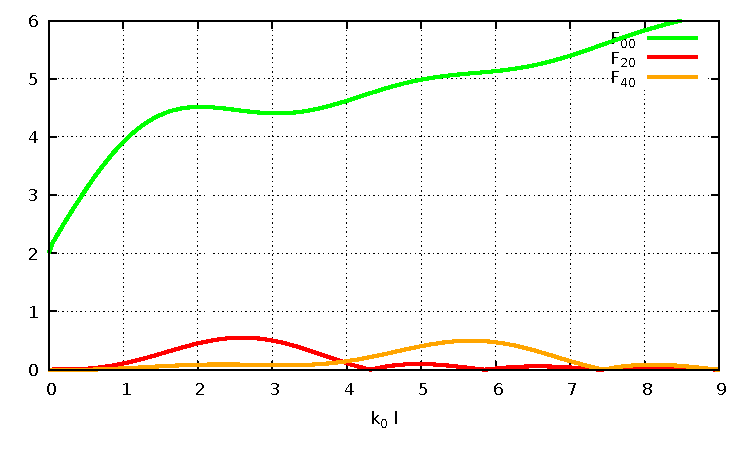
\includegraphics[width = \textwidth]{figures/F00.pdf}
    \caption{Величина модулей матричных элементов $F_{00}$, $F_{20}$ и $F_{40}$ в зависимости от ширины щели.}
    \label{fig:mat_el_00}
\end{figure}

\subsubsection{Предельный переход к идеальному проводнику}
Рассматриваемая в данной работе задача уже была решена для идеального проводника в работах~\cite{gorkunov2011transmission,Shapiro16}, таким образом полученная система уравнений должна переходить в систему для идеального проводника при $\eps \to -\infty$. 

При стремлении $\eps \to -\infty$, второй член под знаком интеграла в~(\ref{eq:F_mn}) стремится к нулю как $\abs{\varepsilon}^{-3/2}$, 
учитывая, что собственные значения антисимметричны $q_{\nu} = -q_{-\nu}$, можно проводить суммирование в уравнении~(\ref{eq:General_System}) 
от $\nu = 0$ до $+\infty$, учитывая каждую моду $\nu \neq 0$ с коэффициентом $2$ (так как для чётных мод $h_\nu = h_{-\nu}$, а для нечётных $h_\nu = -h_{-\nu}$). В итоге, предельный переход даёт ту же систему
уравнений что в работе~\cite{Shapiro16} (подробнее см. Приложение А).

\section{Вклад высших мод при нормальном падении}

Для начала мы сравним результаты для реального и идеального металлов. Выбрав значение проницаемости $\eps = -100 + 10i$, которая соответствует 
проницаемости золота при $\lambda = 1.5$ мкм~\cite{johnson1972optical}, мы вычисляем значение амплитуды магнитного поля на входе в зазор $\abs{H(0,0)}^2$ в зависимости от 
безразмерной ширины $k_0 \ell$ в случае нормального падения излучения. Эта величина примечательна для анализа, потому что по ней можно судить, в какой момент какая мода начинает давать значимый вклад, будь она эванесцентная или распространяющаяся, так как на входе в щель ни одна эванесцентная мода ещё не затухла. 

В работе~\cite{Shapiro16} было показано, что при 
$k_0 \ell \sim 1$ достаточно учитывать лишь две высшие моды, поэтому мы вычисляем лишь значения $h_0$ и $h_2$, не учитывая высшие моды в системе уравнений~(\ref{eq:General_System}).
\begin{figure}
  \begin{subfigure}[t]{1\textwidth}
    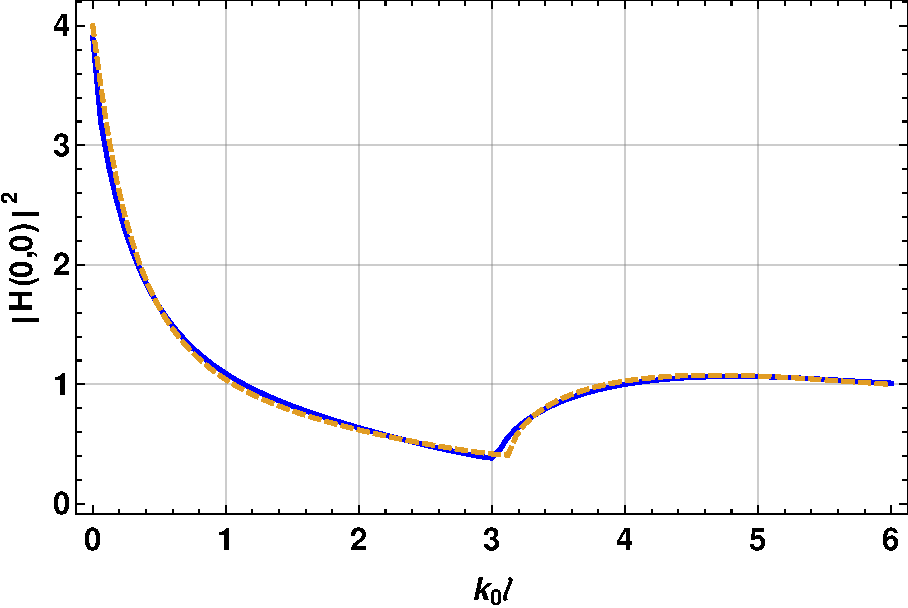
\includegraphics[width=1\textwidth]{H00_2modes_com.pdf}
    \caption{}
  \end{subfigure}
  
  \begin{subfigure}[t]{1\textwidth}
    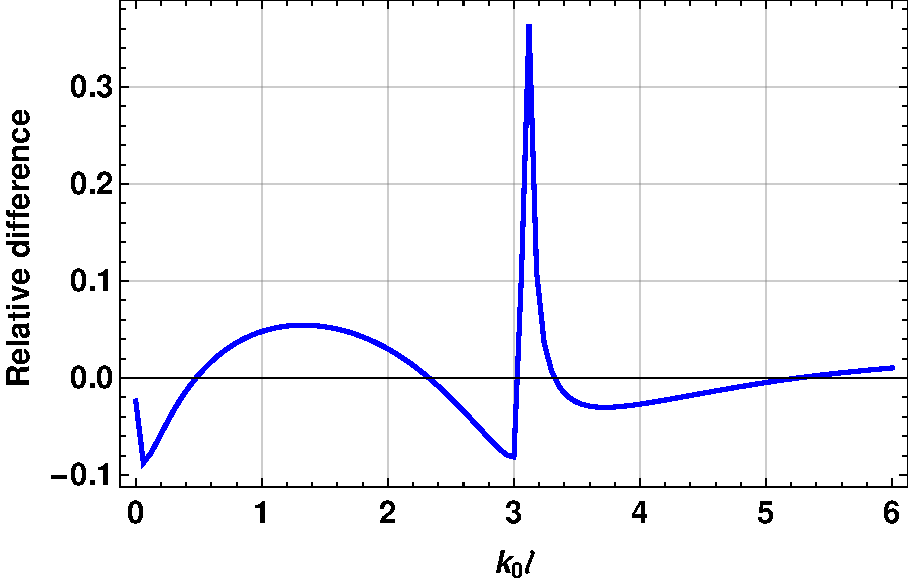
\includegraphics[width=1\columnwidth]{H00_2modes_comp_rel.pdf}
    \caption{}
  \end{subfigure}
  \caption{(a) Зависимость $\abs{H(0,0)}^2$ от $k_0 \ell$. Сплошная линия соответствует конечному $\eps$, пунктир идеальному проводнику. (b) Относительная разница.}	\label{pic:comp}
\end{figure}
На Рис.~\ref{pic:comp} показана зависимость $\abs{H(0,0)}^2$ от $k_0 \ell$ в сравнении с идеальным проводником. Можно заметить, что в целом 
относительная разница не превышает  $10\%$ и лишь при  $k_0 \ell \approx \pi$ достигает $40\%$. Физически эта точка 
соответствует порогу рождения второй моды, а порог рождения, как было показано выше, <<смещается>> при учёте конечной проводимости, и фактически
вблизи этой точки возникает ситуация, когда вторая мода для реального металла уже становится распространяющейся (Рис.~\ref{fig:betta2}), 
в то время как для идеально проводника
она ещё остаётся эванесцентной, отсюда и происходит такая большая разница. Однако стоит заметить, что в целом картина сохраняется,
и учёт конечной проводимости в расчёте амплитуд $h_\nu$ даёт ответ, отличающийся не больше чем на $10\%$, но с другой стороны, этот учёт 
становится дорогостоящим с точки зрения численного интегрирования  коэффициентов в системе линейных уравнений~(\ref{eq:General_System}).

Посчитаем возникающую силу. Так как учитываются две моды, то в тензор Максвелла будет вклад трёх членов
\begin{equation}
  \sigma_{xx}(z) = \sigma_{xx}^0(z)+ \sigma_{xx}^2(z)  + \sigma_{xx}^{02}(z),
\end{equation}
где они определены следующим образом:
\begin{align}
\sigma_{xx}^{0}(z) = \frac{1}{4 \pi k_0^2}\Bigl[\abs{\beta_{0} h_{0} \cos(q_{0}\ell) e^{i \beta_{0} z}}^2   
-\abs{q_{0} h_{0}(z) \sin(q_{0}\ell) e^{i \beta_{0} z}}^2 \nonumber \\
- k_0^2\abs{ h_{0}(z) \cos(q_{0} l) e^{i \beta_{0} z}}^2\Bigr],\nonumber\\
\sigma_{xx}^{2}(z) = \frac{1}{\pi k_0^2}\Bigl[\abs{\beta_{2} h_{2} \cos(q_{2}\ell) e^{i \beta_{2} z}}^2
-\abs{q_{2} h_{2}(z) \sin(q_{2}\ell) e^{i \beta_{2} z}}^2 \nonumber \\
- k_0^2\abs{ h_{2}(z) \cos(q_{2}\ell) e^{i \beta_{2} z}}^2\Bigr],\nonumber\\
\sigma_{xx}^{02}(z) = \frac{1}{ \pi k_0^2} \Re\Bigl[  \beta_0 h_0 \cos(q_0\ell) e^{i \beta_0 z} \cdot \big(\beta_2 h_2 \cos(q_2\ell) e^{i \beta_2 z}\big)^{*}\nonumber\\
- q_0 h_0 \sin(q_0\ell) e^{i \beta_0 z} \cdot \big(q_2 h_2 \sin(q_2\ell) e^{i \beta_2 z}\big)^{*}\nonumber&\\
- k_0^2 h_0 \cos(q_0\ell) e^{i \beta_0 z} \cdot \big(h_2 \cos(q_2\ell) e^{i \beta_2 z}\big)^{*}\Bigr].&\nonumber
\end{align}
Члены $\sigma_{xx}^{0}, \sigma_{xx}^{2}$ определяют давление фундаментальной и второй моды, $\sigma_{xx}^{02}$  --- интерференционный член, * обозначает комплексное сопряжение. Следует отметить, что мода $h_2$ учитывается дважды, так как $h_2 = h_{-2}$.

\begin{figure}
  \begin{subfigure}[t]{0.75\textwidth}
    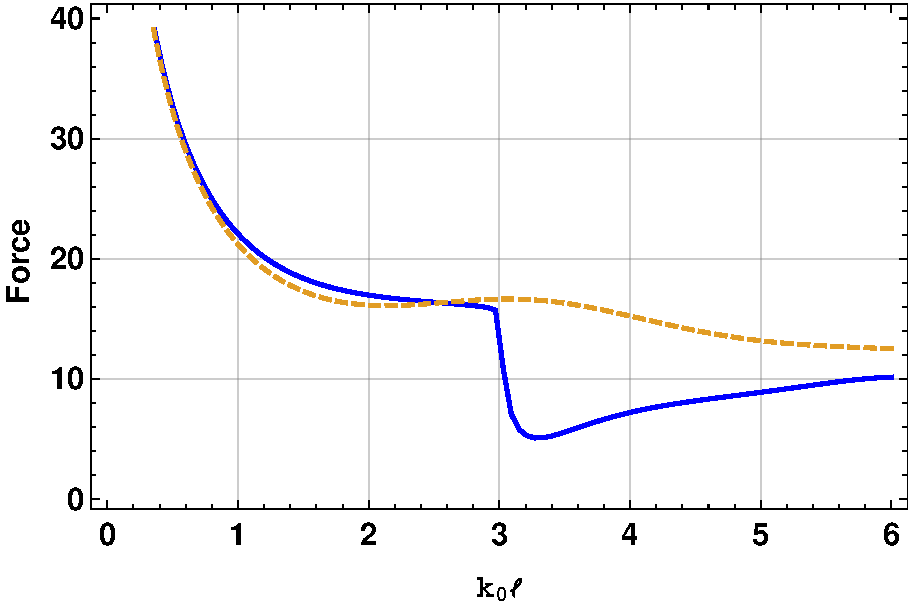
\includegraphics[width=1\columnwidth]{Force.pdf}
    \caption{}
  \end{subfigure}
  \begin{subfigure}[t]{0.75\textwidth}
    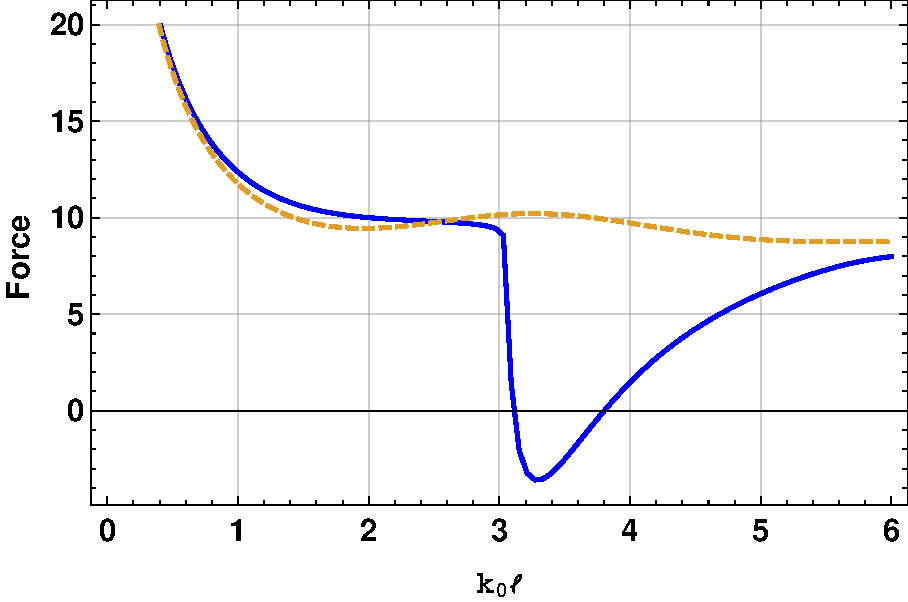
\includegraphics[width=1\columnwidth]{Force_2.pdf}
    \caption{}
  \end{subfigure}
  \caption{Сила между пластинами в условных единицах как функция  $k_0 \ell$. Штрихи --- одна мода, сплошная линия --- две моды: (a) $\eps=-100+10i$, (b) $\eps = -360 + 60i$.}
  \label{fig:F}
\end{figure}

Интегрируя по поверхности пластины, получаем силу на единицу длины:
\begin{equation}
  F \approx \frac{\sigma_{xx}^0(0)}{2 \beta_0^{''}} + \frac{\sigma_{xx}^2(0)}{2 \beta_2^{''}} + \int_{0}^{\infty}\sigma_{xx}^{02}(z)dz,
\end{equation}
где $\beta_{0,2}'=\Re(\beta_{0,2})$ и $\beta_{0,2}''=\Im(\beta_ {0,2 })$. Мы не пишем явное выражение для интерференционного члена из-за его громоздкости, однако легко проверить, что он будет обратнопропорционален разности констант распространения нулевой и второй мод. $L_z$ --- длина вдоль оси $z$ здесь не рассматривается, поскольку мы предполагаем, что $L_z\gg1/\beta_{0,2}''$, что означает, что мы не учитываем отражение мод от верхней границы $(z = L_z)$. Как мы уже отмечали выше, мнимая часть $\beta_i$ определяет глубину проникновения моды $i = 0,2$, а также силу между стенками, а для больших $L_z$ амплитуда $i$-й моды будет уменьшаться экспоненциально, поэтому достаточно рассмотреть только распространяющиеся моды.
 
 Мы рассчитали силу численно в одно- и двухмодовом приближениях. Рис.~\ref{fig:F}(a), соответствующий $\lambda = 1.5$ мкм, показывает, что если $k_0\ell <\pi$
(когда вторая мода является эванесцентной), достаточно принять во внимание только фундаментальную моду. В главе 1 получено аналитическое выражение для одномодового режима~(\ref{eq:F_fund_mode_SGS}),  куда входит только амплитуда $h_0$. Для субволновой щели,чтобы получить аналитическое выражение для силы, можно использовать выражение для $h_0$, полученное в работе~\cite{Shapiro16} для идеального проводника
\begin{equation}
    h_0 = \frac{2}{1 + k_0\ell\Big( (1 - (k_0\ell)^2/6) -i(\alpha_1 + \alpha_2 (k_0\ell)^2)  \Big)}
\end{equation}
со значениями $\alpha_1 = 0.59 - 0.64\log{k_0 \ell}$ и $\alpha_2 = -0.11(1-\log{k_0 \ell})$.
Это приближение разумно применять вплоть до $k_0 \ell=1$ с точностью $10\%$. 
Однако с увеличением ширины щели происходит рождение второй чётной моды, которая имеет решающее значение в величине силы и приводит к трехкратному резкому её снижению. 

Можно заметить, что разные значения $\eps'$ и $\eps''$ могут привести не только к уменьшению силы, но и к изменению ее знака с притягивающей на отталкивающую. Например, на длине волны $\lambda = 3.1$ мкм (соответствующий волновой вектор $k_0 = 2.0~\text{мкм}^{-1}$) диэлектрическая проницаемость золота равна $\eps = -360 + 60i$ \cite{Palik98}. Рис.~\ref{fig:F}(b) показывает, что появление второй моды приводит к отталкиванию в диапазоне $3.1 <k_0\ell<3.8$,
там можно увидеть две точки равновесия, где сила равна нулю. Причём, правая ($k_0 \ell \approx 3.8$) является точкой устойчивого равновесия для пластин, где
в  принципе можно зарегистрировать явление осцилляций. 

\section{Наклонное падение}

Учёт наклонного падения происходит подобно вкладу высших мод. Единственная разница лишь в том, что уравнения для чётных и нечётных мод расцепляются, а значит соответствующие амплитуды $h_\nu$ вычисляются независимо. Для простоты вновь будем рассматривать щель, достаточно узкую  для того, чтобы учитывать только первые четную и нечётную моды. Так как уравнения расцепились, то можно компактно выписать значения амплитуд

\begin{eqnarray}
  h_0 = \frac{(1+R)f_{q_0,k_{0x}} + \ell k_{0z}(1-R)/\pi \int \frac{\sinc((k_{0x}-k)\ell) f_{q_0,k} }{\kappa} dk }{F_{00} } \\
  h_1 = \frac{(1+R)f_{q_1,-k_{0x}} + \ell k_{0z}(1-R)/\pi \int \frac{\sinc((k_{0x}-k)\ell) f_{q_1,-k} }{\kappa} dk }{2F_{11}}
\end{eqnarray}
Отсюда можно оценить влияние угла падения на величину силы. Если $\gamma\ll 1$, то можно оценить амплитуды в случае идеального проводника $q_0 \ell \to 0$, $q_1 \ell \to \pi/2$:
$h_0 \approx 2-(k_0\ell \gamma)^2/3,~h_1 \approx  2 i  k_0\ell \gamma$. Отсюда амплитуда $h_1\sim \gamma$, тогда как поправка к $h_0$ --- порядка $\gamma^2$. Тогда в тензор Максвелла поправка к вкладу от нулевой моды и вклад от первой нечётной будут квадратичными по $\gamma$, в то время как интерференционной член будет первого порядка. 
Конкретные численные расчёты представлены ниже для углов падения $\gamma = 0.01,\ 0.1,\ 1$ радиан.
\begin{figure}
    \centering
    \begin{subfigure}[t]{0.45\textwidth}
        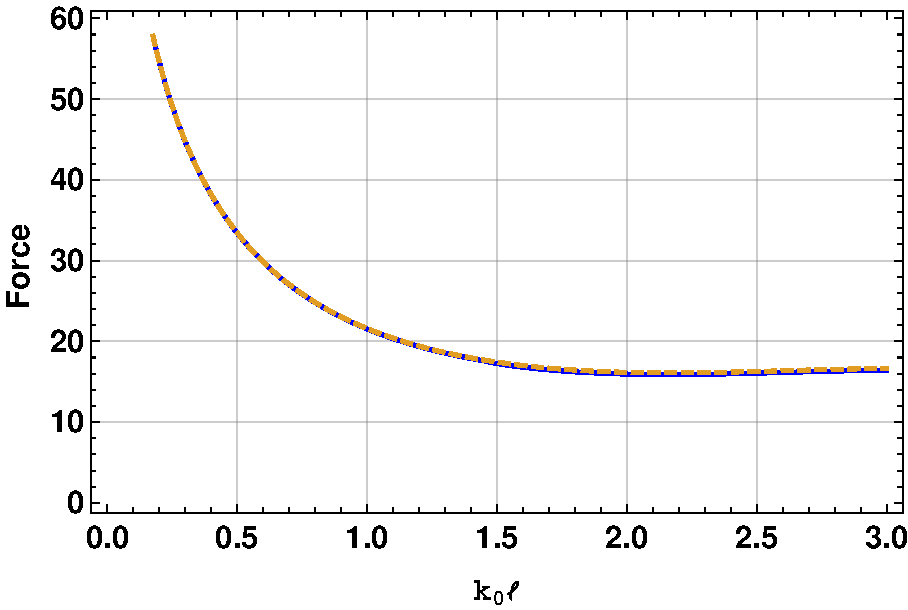
\includegraphics[width=\textwidth]{figures/Force100_001.pdf}
        \caption{}  
        \end{subfigure}
    \begin{subfigure}[t]{0.45\textwidth}
        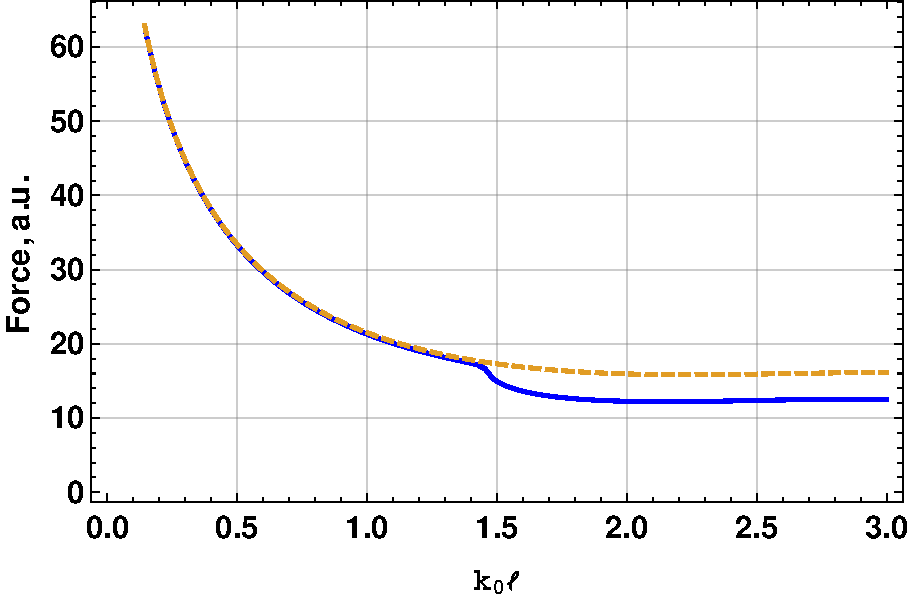
\includegraphics[width=\textwidth]{figures/Force100_01.pdf}
        \caption{}  
    \end{subfigure}
    \begin{subfigure}[t]{0.6\textwidth}
        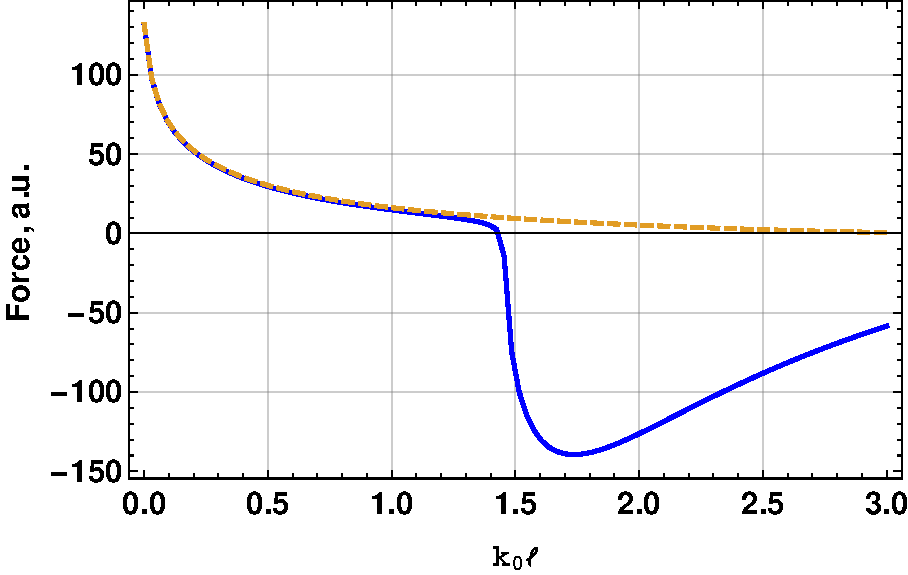
\includegraphics[width=\textwidth]{figures/Force100_1.pdf}
        \caption{}  
    \end{subfigure}
    \caption{Зависимость плазмонной силы в условных единицах от ширины щели для золота при наклонном падении плоской волны: (a) $\gamma = 0.01$, (b) $\gamma = 0.1$, (c)  $\gamma = 1$ радиан.}
    \label{fig:Force100_angle}
\end{figure}

Полученный результат похож на предыдущий: вплоть до порога рождения нечётной моды, основной вклад в плазмонную силу имеет нулевая мода, однако как только нечётная мода становится распространяющейся, при увеличении угла падения, сила меняет знак, и при больших углах падения её величина по модулю сопоставима с силой притяжения при $k_0 \ell \ll 1$. Для эксперимента отклонение $\gamma$ от нуля является неточностью юстировки, и поэтому в эксперименте характерны $\gamma \ll 1$. Выше мы уже показали, что вклад должен быть порядка $\gamma$, прямой расчёт показывает, что при $\gamma = 0.01$ радиан, вклад нечётной гармоники мал.

\section{Учёт конечных размеров пучка}

Рассмотрим в этом разделе фокусировку пучка по оси $x$ при нормальном падении. Предположим, что падающий пучок описывается выражением
\begin{equation}
    H(x,z) = F(x,z)e^{i k_0 z},
\end{equation}
где $F(x,z)$ --- медленная огибающая. Обозначим её при $z = 0$ за $F(x)$ и найдём поля во всём пространстве. Для этого в уравнениях~(\ref{eq:H}) и~(\ref{eq:Ex_in}) нужно заменить член $e^{i k_{0_{x}}x}$ на $F(x)$. Тогда амплитуды $a_k$ через $h_\nu$ будут выражаться следующим образом
\begin{equation}
    a_k = \frac{k_0}{ 2\pi \varkappa} (1-R)\int_{-\ell}^\ell F(x) e^{-ikx}dx - \frac{\ell}{2 \pi \varkappa}\sum_{\nu = -\infty}^{+\infty} \beta_\nu h_\nu\left[f_{q_\nu,k}
+ \frac{m_\nu(\ell)}{\eps}G(q_\nu,k)\right].
\label{eq:ak_F(x)}
\end{equation}
Введём обозначение $\int_{-\ell}^\ell F(x) e^{-ikx}dx \equiv 2\ell \hat{F}(k,\ell)$, тогда получаем систему уравнений на $h_\nu$ 
\begin{align}
	\sum_{\nu=-\infty}^{+\infty} F_{\mu \nu} h_\nu = \frac{(1+R)}{\ell}\int_{-\ell}^\ell F(x) m_\mu(x)dx + \frac{(1-R)k_{0} l}{\pi}\int f_{q_\mu,-k}\hat{F}(k,\ell) \frac{dk}{\varkappa}, \label{eq:General_System_F(x)}
\end{align}
или в матричной форме
\begin{equation}
    \mathcal{F} h = b.
    \label{eq:matrix_form_F(x)}
\end{equation}
Здесь сохраняются те же обозначения, что были использованы выше. Заметим, что рассмотренный выше случай падения плоской волны под произвольным углом --- это частный случай полученной системы~(\ref{eq:General_System_F(x)}), так как в случае наклонного падения волны $F(x) = e^{i k_{0_x}x}$, и тогда $\hat{F}(k,\ell) = \text{sinc}((k_{0_x} - k)\ell)$ и $\int_{-\ell}^\ell F(x) m_\mu(x)dx/\ell = f_{q_\mu,-k_{0_x}}$.

Введение огибающей не вносит больших изменений в систему уравнений~(\ref{eq:General_System}), так как матричные элементы $F_{\mu \nu}$, которые описывают связь между модами $\mu$ и $\nu$, зависят только от длины волны падающего излучения, ширины щели и диэлектрической проницаемости. Форма фронта входит в правую часть системы уравнений, и как уже было показано, при нормальном падении плоской волны возбуждаются лишь чётные моды, при отклонении вектора падения от нормали, начинают возбуждаться нечётные моды. Однако вклад в силу вносят только распространяющиеся моды. Здесь, по сути, такая же ситуация, и определять силу будут лишь распространяющиеся моды. 

Предположим, что фронт имеет гауссов профиль при $z = 0$
\begin{equation}
    F(x) = e^{-\frac{x^2}{w_0^2}}.
\end{equation}
Тогда доминирующий член по $\eps$ в правой части~(\ref{eq:General_System_F(x)}) будет равен
    \begin{align}
    \frac{(1+R)}{\ell}\int_{-\ell}^\ell F(x) \cos(q_\mu x) dx =& \nonumber \\ \frac{\sqrt{\pi}(1+R)}{2}\frac{w_0}{\ell}e^{-\frac{q_\mu^2 w_0^2}{4}} & \Bigg( \text{Erf}\Big(\frac{\ell}{w_0} - \frac{i q_\mu w_0}{2 \ell}\Big) + \text{Erf}\Big(\frac{\ell}{w_0} + \frac{i q_\mu w_0}{2 \ell}\Big) \Bigg).
\end{align}
\begin{figure}
    \centering
    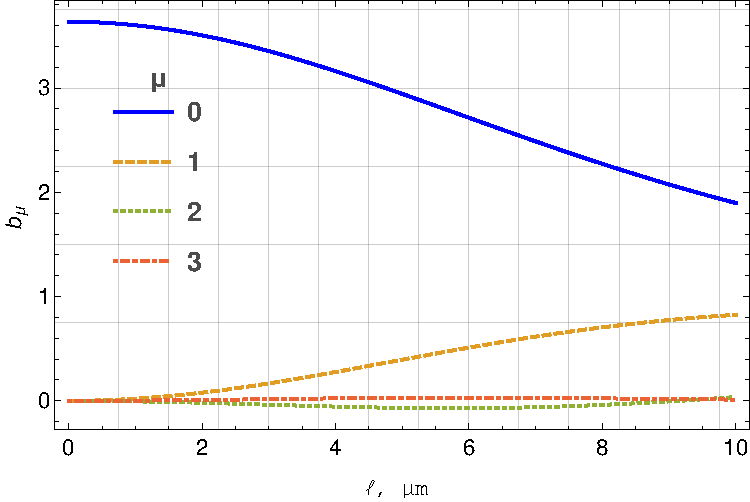
\includegraphics[width = \textwidth]{figures/Bm.pdf}
    \caption{Зависимость компонент правой части $b_\mu$ уравнения~(\ref{eq:matrix_form_F(x)}) для фундаментальной $\mu = 0$ и последующих чётных мод $\mu = 1,\ 2,\ 3$ от ширины щели. Вертикальные линии сетки соответствуют порогам рождения чётных мод.}
    \label{fig:b_mu_F(x)}
\end{figure}
Отсюда видно, что вклад высших мод экспоненциально подавлен. Прямой расчёт этого выражения для $\lambda = 1.5$ мкм и $w_0 = 4 \lambda$ для различных возбуждаемых мод представлен на Рис.~\ref{fig:b_mu_F(x)}. Вертикальные линии сетки на графике соответствуют порогам рождения чётных мод. Вплоть до порога рождения третьей чётной моды вклад фокусировки в первую моду незначителен, и тогда падающее излучение можно считать плоской волной. В этой области тогда можно записать правую часть системы уравнений~(\ref{eq:matrix_form_F(x)}) в приближённой форме
\begin{equation}
    b_\mu \approx \delta_{\mu,0}\frac{(1+R)}{2}(4 - \frac{4 \ell^2}{3 w_0^2}).
    \label{eq:b0_F(x)_approx}
\end{equation}

На Рис.~\ref{fig:Force_PW_Gauss_100_10} представлено сравнение между силами при падении плоской волны и сфокусированного пучка для проницаемости золота $-100 + 10i$. Расчёт подтверждает, что вплоть до порога рождения второй чётной моды разница между возникающими силами незначительная, однако после рождения второй чётной моды она увеличивается. Величина силы для сфокусированного пучка немного уменьшается. Причина такого поведения видна из графиков на Рис.~\ref{fig:h0_pw_gauss} и~\ref{fig:h24_pw_gauss}. При увеличении ширины щели амплитуда $h_0$ уменьшается, по сравнению со случаем падения плоской волны, что согласуется с~(\ref{eq:b0_F(x)_approx}). Однако амплитуда второй гармоники становится заметно больше с ростом ширины, в то время как влияние профиля фронта практически никак не сказывается на четвёртой моде.
\begin{figure}
    \centering
    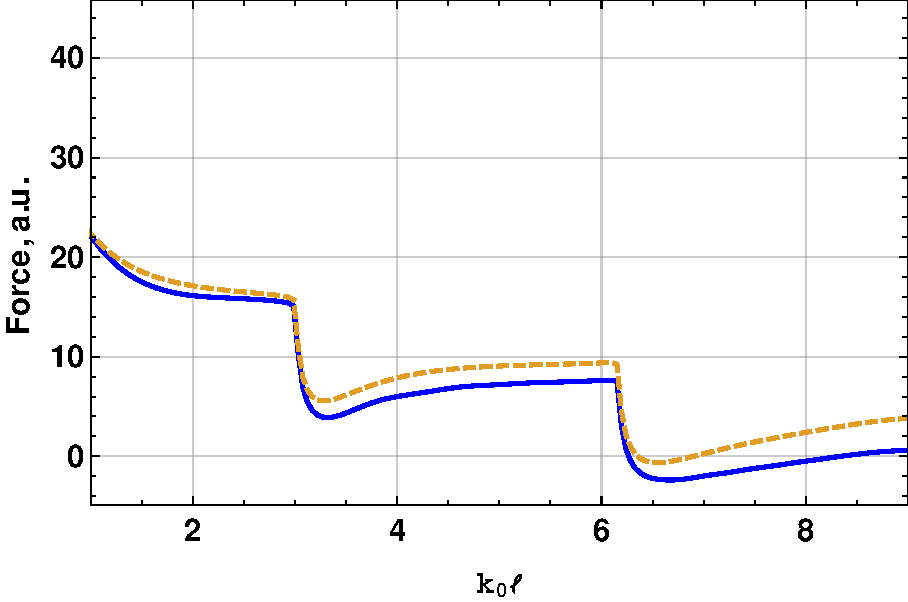
\includegraphics[width=\textwidth]{figures/Force_PW_GAUSS.pdf}
    \caption{Сила между пластинами в условных единицах в зависимости от безразмерной ширины щели в случае падения фокусированного пучка (сплошная линия) и плоской волны (пунктир).}
    \label{fig:Force_PW_Gauss_100_10}
\end{figure}

\begin{figure}
    \centering
    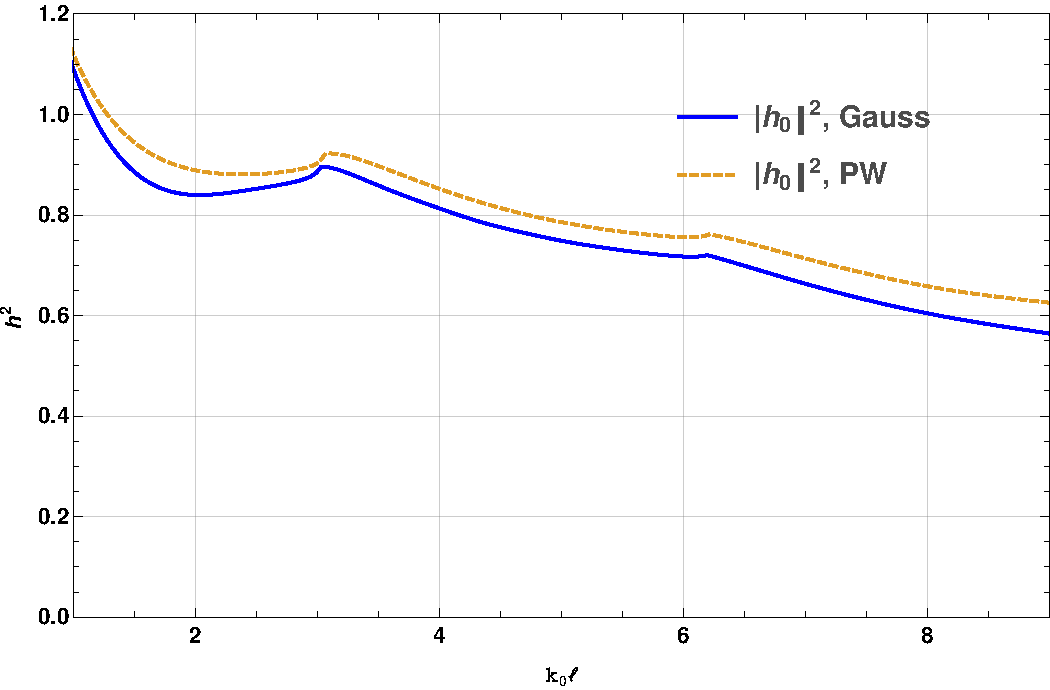
\includegraphics[width=\textwidth]{figures/h0_PW_GAUSS.pdf}
    \caption{Величина квадрата модуля амплитуды фундаментальной моды в зависимости от $k_0 \ell$ при падении плоской волны (PW) и сфокусированного пучка (Gauss).}
    \label{fig:h0_pw_gauss}
\end{figure}
\begin{figure}
    \centering
    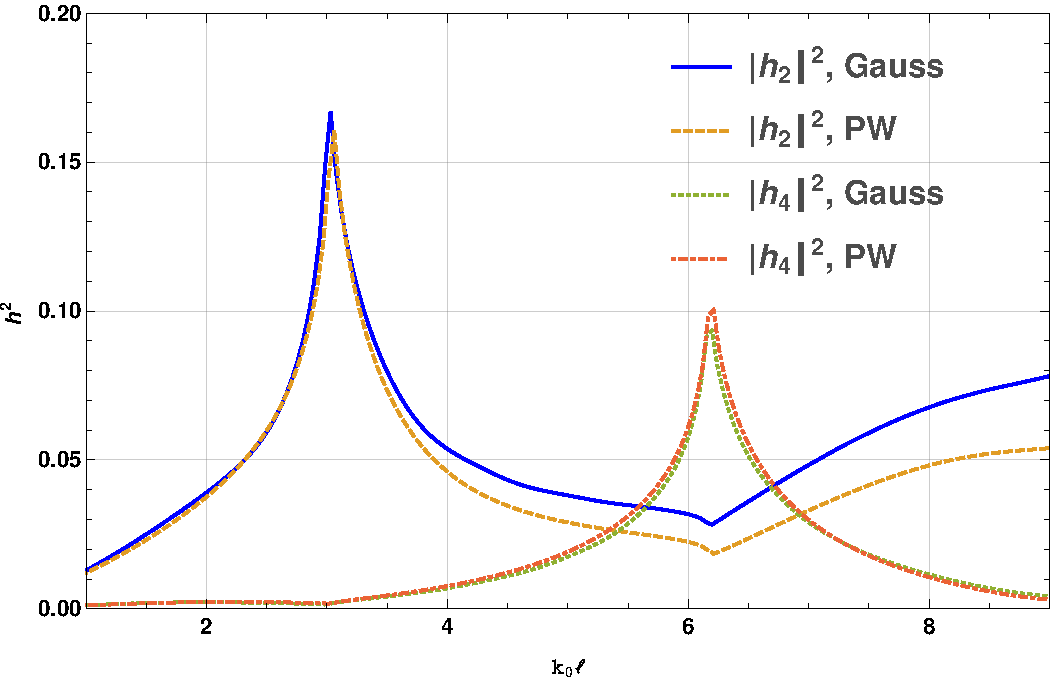
\includegraphics[width=\textwidth]{figures/h24_PW_GAUSS.pdf}
    \caption{Величина квадрата модуля амплитуды второй и четвёртой мод в зависимости от $k_0 \ell$ при падении плоской волны (PW) и сфокусированного пучка (Gauss).}
    \label{fig:h24_pw_gauss}
\end{figure}
\section{Численное моделирование}
Для проверки представленной теории было произведено моделирование двумерной задачи в программном пакете Comsol Multiphysics с использованием модуля Radio Frequency (RF), который решает уравнения Максвелла методом конечных элементов (МКЭ).

Среди численных методов МКЭ один из самых широкоиспользуемых методов для решения уравнений в частных производных в широком спектре исследовательских и научно-прикладных задач~\cite{zenkevich}. Одним из его достоинств является то, что он позволяет решить задачу в произвольной геометрии, а матрицы, получающиеся в процессе дискретизации, являются разреженными (sparse)~\cite{zienkiewicz2005finite}, что позволяет экономить память для хранения матриц и использовать специальные алгоритмы, ускоряющие алгебраические операции над матрицами. Например, в методе граничных элементов, который требует дискретизации лишь границы объектов, на которых происходит рассеяние, получаемые матрицы получаются полностью заполненными (dense), что накладывает повышенные требования (по сравнению с МКЭ) на вычислительные ресурсы~\cite{marburg2008computational}.

Для решения поставленной задачи использовался модуль Frequency Domain в модуле RF, который решает уравнение
\begin{equation}
    \text{rot}(\text{rot}\mathbf{E}) - \varepsilon k_0^2 \mathbf{E} = 0.
    \label{eq:Helmholtz_rot}
\end{equation}
Особенность МКЭ заключается в том, что теоремы о сходимости численных решений (например теорема Лакса-Милграмма) формулируются для ограниченных областей~\cite{ciarlet2002finite}. В данной работе рассматривается задача с открытыми границами, поэтому было необходимо смоделировать бесконечность. Для этого использовались идеально согласованные слои PML (от англ. Perfectly Matched Layers), в которых падающая волна поглощается, не отражаясь от границы с расчётной областью~\cite{comsol_book}. Таким образом, мы окружили расчётную область поглощающими слоями со всех сторон. Расположение расчётной области золота, воздуха и PML слоёв представлены на Рис.~\ref{fig:Comp_dom}. Так как в золоте волновой вектор в $\sqrt{\varepsilon} \sim 10$ раз больше, чем в воздухе, мы использовали более грубое разбиение расчётной области в золоте вдали от границы, чтобы сэкономить расчётные ресурсы. 

\begin{figure}
    \begin{subfigure}[t]{\textwidth}
        \centering
        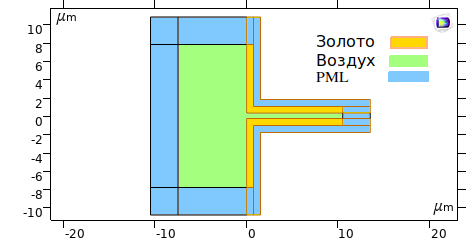
\includegraphics[width=\textwidth]{figures/Geometry2_gold.png}
        \caption{}
    \end{subfigure}
    \begin{subfigure}[t]{\textwidth}
        \centering
        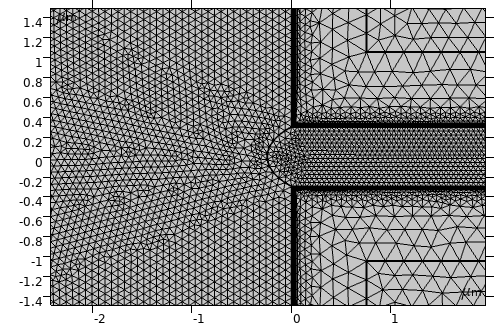
\includegraphics[width=\textwidth]{figures/mesh.png}
        \caption{}
    \end{subfigure}
        \caption{Геометрия задачи в моделировании. (a) Рассчётная область, (b) разбиение расчётной области вблизи входа в щель.}
        \label{fig:Comp_dom}
\end{figure}

Мы проводили численный эксперимент в условиях нормального падения плоской волны на щель с амплитудой электрического поля $1$ В/м.
Результаты моделирования представлены на графиках ниже. На Рис.~\ref{fig:Hz_cut_z} представлено распределение модуля магнитного поля на срезе $z = 1.5$ мкм при полуширине щели $\ell=0.5$ мкм. Точками изображено моделирование COMSOL, кривой --- аналитическое распределение поля в одномодовом приближении. Ранее мы уже получали, что при $k_0 \ell < \pi$ одномодовое приближение хорошо работает, и как следствие, при удалении от входа в щель должна быть только нулевая мода, а следовательно, внутри щели это должна быть цепная линия с параметром $q_0$, определяемым дисперсионным уравнением~(\ref{eq:BoundCond}), а в золоте должны быть затухающие экспоненты. Моделирование COMSOL соответствует этой картине  и воспроизводит результат работы~\cite{sturman2007eigenmodes} для единственной распространяющейся моды в субволновой щели. На Рис.~\ref{fig:Hz_005} представлен срез $\abs{H(x =0,z)}^2$. Как уже оговаривалось, в узкой щели модуль поля должен экспоненциально затухать с показателем $\beta_0''$, численное моделирование подтверждает этот результат. То же получается и для других мод. 

\begin{figure}
    \centering
    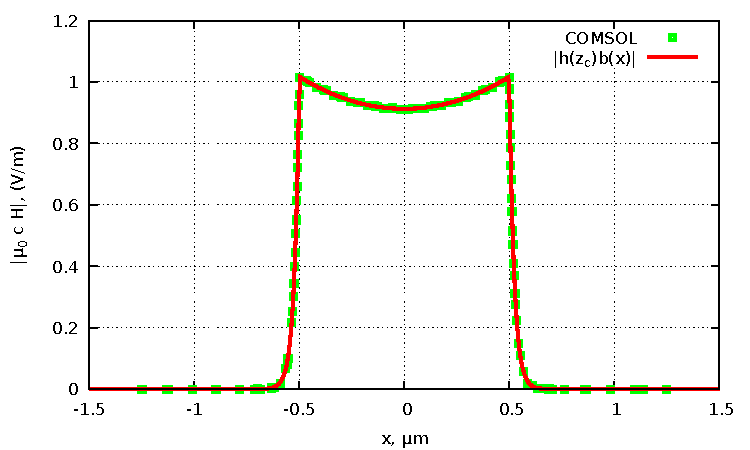
\includegraphics[width=\textwidth]{figures/Hz_cut.pdf}
    \caption{Модуль магнитного поля в срезе $z=1.5$ мкм, $\ell = 0.5$ мкм. Пунктир --- моделирование COMSOL, непрерывная линия --- аналитическое решение. }
    \label{fig:Hz_cut_z}
\end{figure}

\begin{figure}
    \centering
    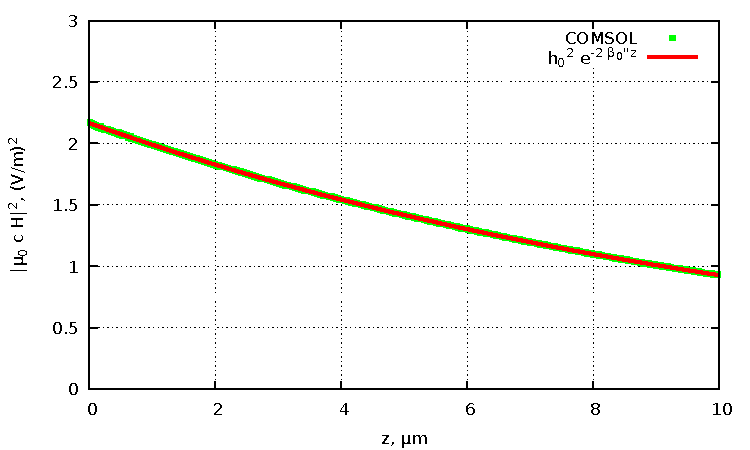
\includegraphics[width=\textwidth]{figures/Hz_005.pdf}
    \caption{$\abs{H(x=0,z)}^2$ при $\ell=0.05$ мкм. Моделирование COMSOL и одномодовое приближение.}
    \label{fig:Hz_005}
\end{figure}

Как было показано выше, собственные значения в щели хорошо воспроизводятся численным моделированием, однако вопрос о том, какие моды возбуждаются падающим излучением остаётся открытым. 
%   В ходе моделирования мы столкнулись с численной сложностью, которая возникает при пересчёте электрического поля, найденного численно из уравнения Гельмгольца~(\ref{eq:Helmholtz_rot}), в магнитное. Тот факт, что в модуле RF используется E-формулировка уравнения Гельмгольца, то есть численно ищется решение для электрического поля, а после пересчитывается магнитное, в некоторых ситуациях порождает поля $H$ на входе в щель. Рис.~\ref{fig:E_cont} демонстрирует, что $x$-компонента поля $E$ непрерывна на входе в щель, однако $H_z$ терпит нефизичный скачок при $z=0$. Так как это численный артефакт, то мы его вручную удаляли и восстанавливали значение поля при $z = 0$ линейной интерполяцией.
%   \begin{figure}
%       \begin{subfigure}[t]{\textwidth}
%           \centering
%           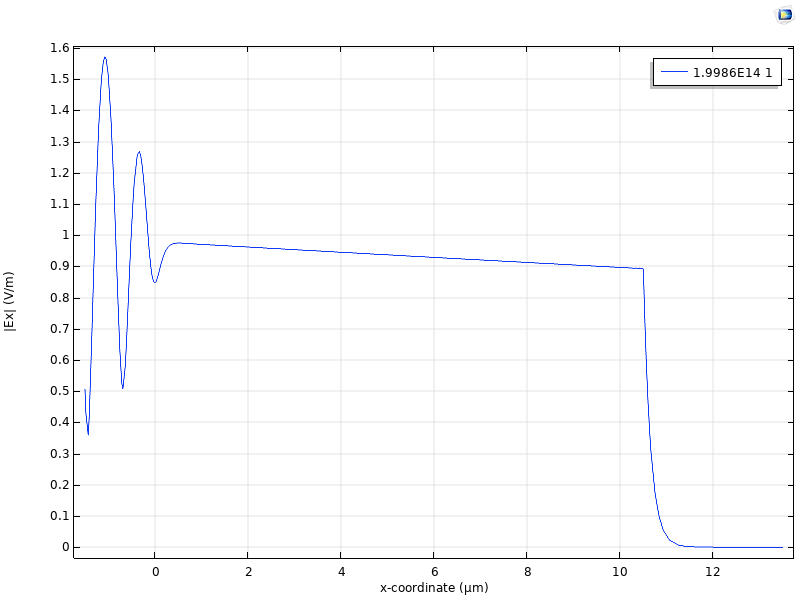
\includegraphics[width=\textwidth]{figures/E.png}
%       \end{subfigure}
%       \begin{subfigure}[t]{\textwidth}
%           \centering
%           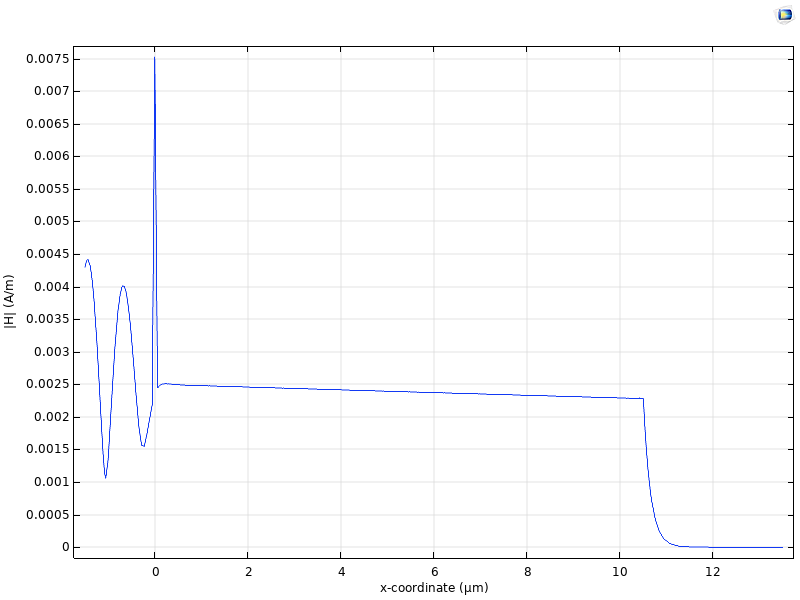
\includegraphics[width=\textwidth]{figures/H_discotunity.png}
%       \end{subfigure}
%       \caption{Зависимость (a) $\abs{E_x(x=0,z)}$ (b)  $\abs{H(x=0,z)}$ от $z$. }
%           \label{fig:E_cont}
%   \end{figure}
Чтобы ответить на этот вопрос было проведено несколько численных экспериментов с разной шириной щели. В результате была получена зависимость $\abs{H(0,0)}^2$ от ширины, которая показывает какие моды возбуждаются при различных ширинах. Эта зависимость представлена на Рис.~\ref{fig:H00_sim_an} в сравнении с теорией в двухмодовом и трёхмодовом приближениях. Численное моделирование повторяет пиловидную структуру, что была предсказана в~\cite{Shapiro16} для идеального проводника, однако всё-таки имеется различие порядка $\sim 10\%$ с теорией. Это может быть связано с тем, что шаг сетки недостаточно маленький. Однако, как уже было показано выше, различные значения проницаемости для золота не дают большой разницы для амплитуд поля, а играют решающую роль в расчёте констант распространения для различных мод, которые определяют силу между пластинами. 
\begin{figure}
    \centering
    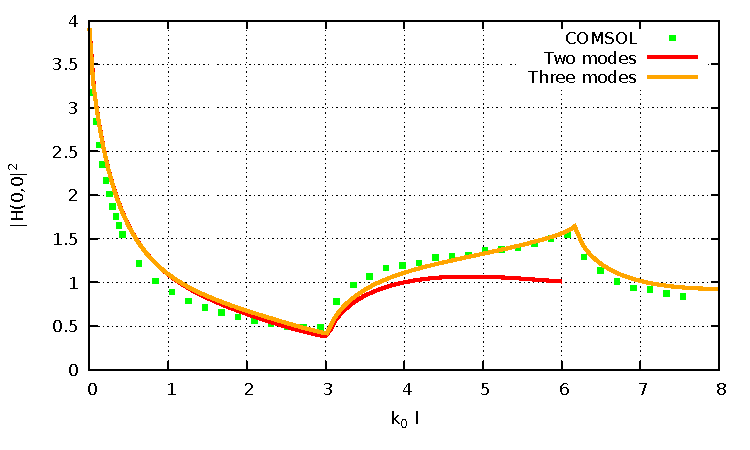
\includegraphics[width=\textwidth]{figures/H00_sim_analytic.pdf}
    \caption{Зависимость квадрата модуля магнитного полня на входе в щель $\abs{H(0,0)}^2$ от ширины щели. Моделирование COMSOL, одномодовое и трёхмодовое приближение.}
    \label{fig:H00_sim_an}
\end{figure}

Один из интересных результатов численного расчёта --- это распределение полей вблизи порога рождения новых мод. На Рис.~\ref{fig:Ex_06-08} видна причина, почему новая распространяющаяся мода приводит к резкому изменению поля на входе щели. При $\ell = 0.6$ мкм вторая чётная мода сосредоточивается у входа, когда $\ell = 0.7$ мкм, она уже заходит в щель, но всё ещё остаётся затухающей. При дальнейшем уширении $\ell=0.75$ мкм виден переходной процесс из затухающей в распространяющуюся моду, а при $\ell = 0.8$ мкм видно, что мода уже точно стала распространяющейся. К тому же, эти графики иллюстрируют, что для моделирования этой задачи лучше представлять область вне щели в виде полукруга, так как отражённые волны имеют близкий к окружности фронт. Этот факт важен для коэффициента отражения для различных типов граничных условий, моделирующих открытые границы (см. Приложение Б).  
\begin{figure}
    \begin{subfigure}[t]{0.4\textwidth}
        \centering
        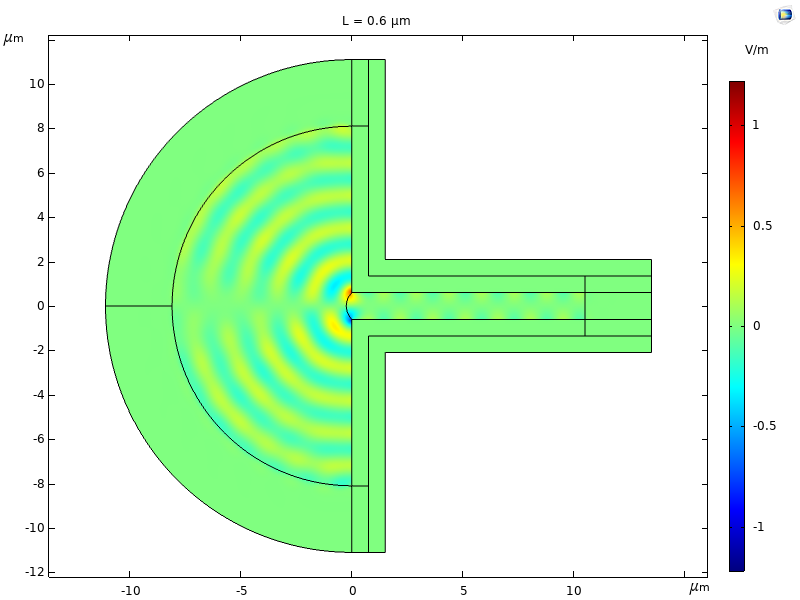
\includegraphics[width=\textwidth]{figures/Ex_06.png}
        \caption{}
    \end{subfigure}
    \begin{subfigure}[t]{0.4\textwidth}
        \centering
        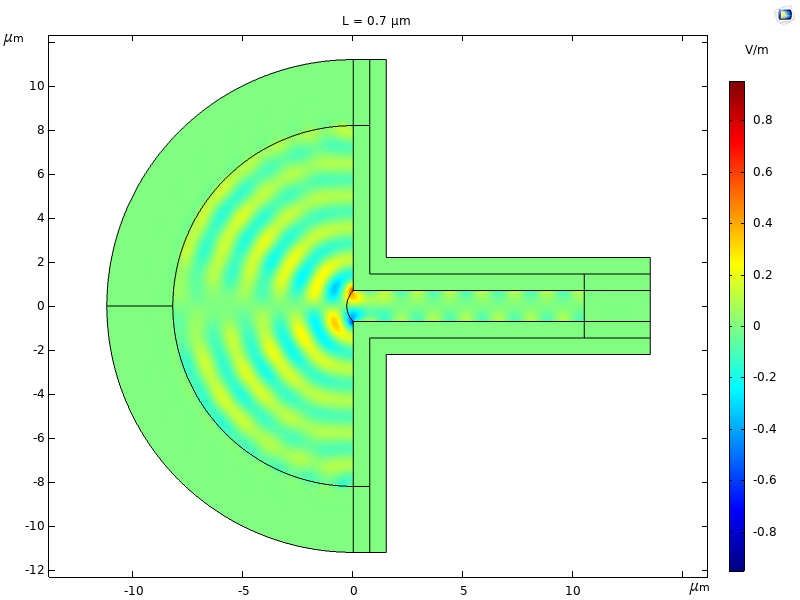
\includegraphics[width=\textwidth]{figures/Ex_07.png}
        \caption{}
    \end{subfigure}
    
    \begin{subfigure}[t]{0.4\textwidth}
        \centering
        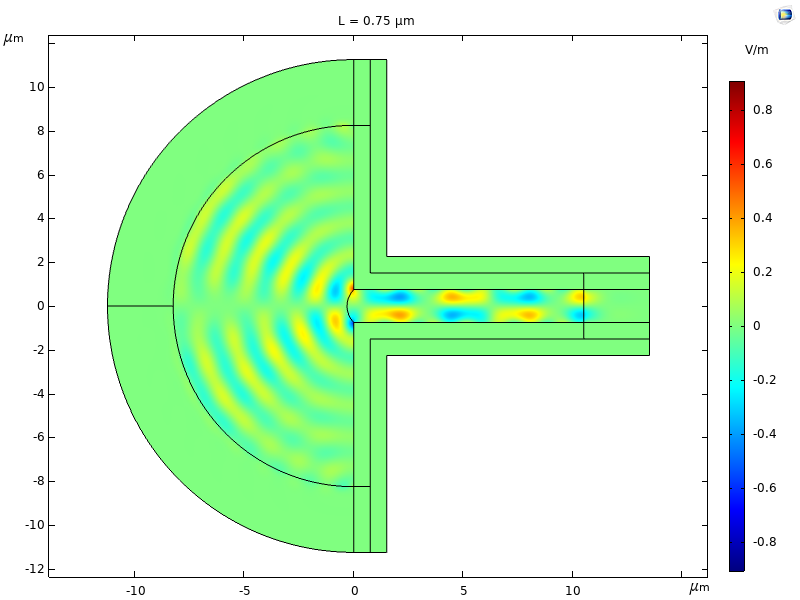
\includegraphics[width=\textwidth]{figures/Ex_075.png}
        \caption{}
    \end{subfigure}
    \begin{subfigure}[t]{0.4\textwidth}
        \centering
        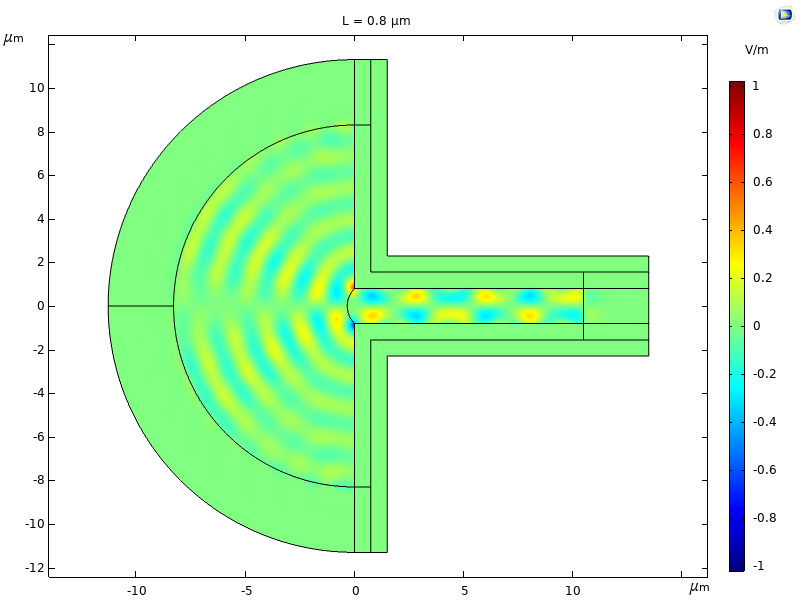
\includegraphics[width=\textwidth]{figures/Ex_08.png}
        \caption{}
        \label{fig:Ex_08}
    \end{subfigure}
    \caption{Распределение z компоненты электрического поля при ширинах щели: (a) $\ell = 0.6$ мкм, (b) $\ell = 0.7$ мкм, (c) $\ell = 0.75$ мкм, (d) $\ell = 0.8$ мкм.}
        \label{fig:Ex_06-08}
\end{figure}



Из моделирования мы можем заключить, что численный расчёт согласуется с теоретическим. В частности, численное моделирование иллюстрирует: 
\begin{itemize}
    \item что можно учитывать лишь распространяющиеся моды в процессе расчёта полей;
    \item рождение распространяющейся моды сопровождается резким изменением амплитуды поля на входе;
    \item хорошее количественное соответствие для констант распространения и амплитуд полей между аналитическим расчётом и численным.
\end{itemize}


